\section{Metody prohledávání stavového prostoru: formulace problému, stavový prostor, strategie prohledávání, neinformované a informované metody (včetně heuristik), kompletnost a optimálnost, příklady problémů v AI.}

\subsection*{Grafy a stavový prostor}
Graf je dvojice
\begin{equation}
    G=(V,E)
\end{equation}
kde \(V\) je množina vrcholů a \(E\) je množina hran.

\begin{itemize}
    \item \textbf{Neorientovaný graf} -- hrana nemá směr, dvojice vrcholů je neuspořádaná.
    \item \textbf{Orientovaný graf} -- hrana má směr, zapisuje se jako uspořádaná dvojice \((u,v)\).
    \item \textbf{Ohodnocený graf} -- hrany mají cenu, např. vzdálenost, čas nebo energii.
\end{itemize}

Ve stavovém prostoru má vrchol význam \textbf{stavu} a hrana význam
\textbf{akce / operátoru}. Cílem prohledávání je najít posloupnost operátorů,
která převede počáteční stav do cílového stavu.

\begin{figure}[H]
    \centering
    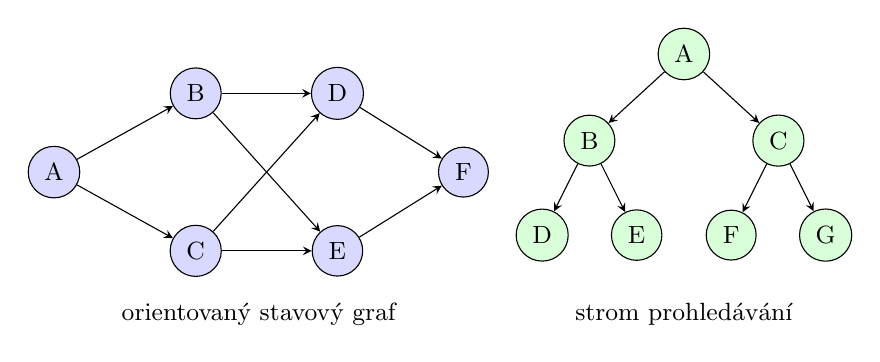
\begin{tikzpicture}[>=stealth, every node/.style={font=\small}]
        \node[draw,circle,fill=blue!15] (a) at (0,1) {A};
        \node[draw,circle,fill=blue!15] (b) at (1.8,2) {B};
        \node[draw,circle,fill=blue!15] (c) at (1.8,0) {C};
        \node[draw,circle,fill=blue!15] (d) at (3.6,2) {D};
        \node[draw,circle,fill=blue!15] (e) at (3.6,0) {E};
        \node[draw,circle,fill=blue!15] (f) at (5.2,1) {F};
        \draw[->] (a)--(b);
        \draw[->] (a)--(c);
        \draw[->] (b)--(d);
        \draw[->] (b)--(e);
        \draw[->] (c)--(d);
        \draw[->] (c)--(e);
        \draw[->] (d)--(f);
        \draw[->] (e)--(f);
        \node at (2.6,-0.8) {orientovaný stavový graf};

        \node[draw,circle,fill=green!15] (s0) at (8,2.5) {A};
        \node[draw,circle,fill=green!15] (s1) at (6.8,1.4) {B};
        \node[draw,circle,fill=green!15] (s2) at (9.2,1.4) {C};
        \node[draw,circle,fill=green!15] (s3) at (6.2,0.2) {D};
        \node[draw,circle,fill=green!15] (s4) at (7.4,0.2) {E};
        \node[draw,circle,fill=green!15] (s5) at (8.6,0.2) {F};
        \node[draw,circle,fill=green!15] (s6) at (9.8,0.2) {G};
        \draw[->] (s0)--(s1);
        \draw[->] (s0)--(s2);
        \draw[->] (s1)--(s3);
        \draw[->] (s1)--(s4);
        \draw[->] (s2)--(s5);
        \draw[->] (s2)--(s6);
        \node at (8,-0.8) {strom prohledávání};
    \end{tikzpicture}
    \caption{Stavový graf zachycuje vztahy mezi stavy, strom prohledávání zachycuje konkrétní rozvoj možností algoritmem.}
\end{figure}

\subsection*{Tah, sled, cesta, strom}
\begin{itemize}
    \item \textbf{Sled} -- libovolný průchod grafem, mohou se opakovat vrcholy i hrany.
    \item \textbf{Tah} -- průchod bez opakování hran.
    \item \textbf{Cesta} -- tah bez opakování vrcholů.
    \item \textbf{Strom} -- souvislý acyklický graf. Má kořen a následníky, neobsahuje cykly.
\end{itemize}

\textbf{Eulerovský tah} projde všechny hrany právě jednou. Eulerovská kružnice je Eulerovský tah, který začíná a končí ve stejném vrcholu.

\textbf{Hamiltonovská cesta} projde všechny vrcholy právě jednou. Hamiltonovská kružnice je uzavřená Hamiltonovská cesta. Rozdíl je důležitý: Euler řeší hrany, Hamilton řeší vrcholy. Hamiltonovské úlohy jsou obecně těžší, typicky NP-těžké.

\subsection*{Reprezentace grafu v paměti}
\begin{itemize}
    \item \textbf{Seznam sousedů} -- ke každému vrcholu seznam dosažitelných sousedů. Úsporné pro řídké grafy.
    \item \textbf{Matice sousednosti} -- tabulka \(n \times n\), rychle zjistí existenci hrany, ale bere hodně paměti.
    \item \textbf{Seznam hran} -- seznam dvojic nebo trojic \((u,v,c)\). Hodí se pro algoritmy pracující přímo s hranami.
\end{itemize}

\subsection*{Formulace problému}
Problém ve stavové reprezentaci se zapisuje pomocí:
\begin{itemize}
    \item počátečního stavu \(s_0\),
    \item množiny operátorů \(A(s)\),
    \item přechodové funkce \(Result(s,a)\),
    \item testu cíle \(Goal(s)\),
    \item ceny přechodu \(c(s,a,s')\).
\end{itemize}

Řešení je plán:
\begin{equation}
    P=(a_1,a_2,\dots,a_n)
\end{equation}
který vytvoří posloupnost stavů od \(s_0\) do cíle.

\textbf{Stavový graf} je mapa celého problému. Každý stav je v něm ideálně jen jednou. \textbf{Strom prohledávání} je dynamická struktura vznikající během běhu algoritmu. Stejný stav se v něm může objevit vícekrát, pokud k němu vedou různé cesty.

\textbf{Hierarchizace stavového prostoru} znamená, že problém nejdříve řešíme zhruba na vyšší abstrakci a teprve potom zpřesňujeme detaily. Zmenšuje prostor hledání a zrychluje plánování, např. u navigace robota.

\subsection*{Obecný princip prohledávání}
Algoritmus drží dvě množiny:
\begin{itemize}
    \item \textbf{OPEN} -- kandidáti, které lze ještě expandovat,
    \item \textbf{CLOSED} -- již zpracované uzly.
\end{itemize}

Expanze znamená, že z vybraného uzlu vygenerujeme jeho následníky. Strategie
určuje, který uzel z OPEN se vybere jako další.

\begin{figure}[H]
    \centering
    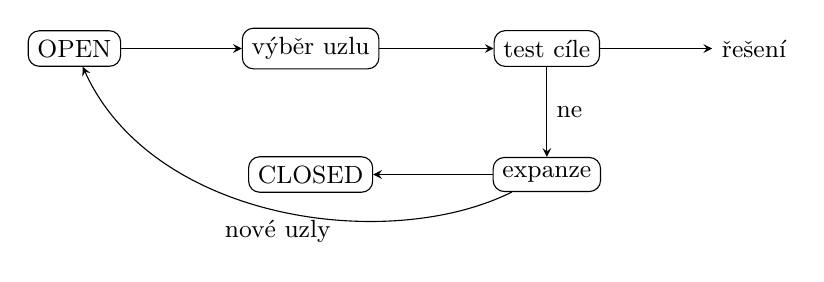
\begin{tikzpicture}[>=stealth, every node/.style={font=\small}]
        \node[draw,rounded corners] (open) at (0,0) {OPEN};
        \node[draw,rounded corners] (select) at (3,0) {výběr uzlu};
        \node[draw,rounded corners] (goal) at (6,0) {test cíle};
        \node[draw,rounded corners] (expand) at (6,-1.6) {expanze};
        \node[draw,rounded corners] (closed) at (3,-1.6) {CLOSED};
        \draw[->] (open)--(select);
        \draw[->] (select)--(goal);
        \draw[->] (goal)--node[right]{ne}(expand);
        \draw[->] (expand)--(closed);
        \draw[->] (expand) .. controls (4,-2.6) and (1,-2.2) .. node[below]{nové uzly} (open);
        \draw[->] (goal) -- ++(2.1,0) node[right]{řešení};
    \end{tikzpicture}
    \caption{Obecný tok prohledávacího algoritmu.}
\end{figure}

\subsection*{Neinformované prohledávání}
Neinformované metody neznají vzdálenost k cíli. Řídí se jen strukturou grafu a
případně cenami hran.

\begin{itemize}
    \item \textbf{BFS} -- prohledávání do šířky, postupně prochází úrovně. Používá frontu. Je paměťově náročné, ale při jednotkových cenách je úplné a optimální.
    \item \textbf{DFS} -- prohledávání do hloubky, jde co nejdál a pak se vrací. Používá zásobník/rekurzi. Má nízkou paměť, ale nemusí být úplné v nekonečném prostoru a není optimální.
    \item \textbf{DLS} -- DFS s hloubkovým limitem. Nezacyklí se do nekonečné hloubky, ale může minout řešení pod limitem.
    \item \textbf{UCS} -- vybírá uzel s nejmenší dosavadní cenou \(g(n)\). Je jako BFS pro různé ceny hran. Při kladných cenách je úplný a optimální.
    \item \textbf{IDDFS} -- opakuje DFS s rostoucím limitem. Paměťově jako DFS, úplností podobné BFS.
\end{itemize}

\begin{center}
    \begin{tabularx}{\textwidth}{|l|X|X|X|}
        \hline
        \textbf{Metoda} & \textbf{Princip}        & \textbf{Úplnost}               & \textbf{Optimálnost} \\
        \hline
        BFS             & po úrovních             & ano pro konečný větvící faktor & ano pro stejné ceny  \\
        \hline
        DFS             & co nejhlouběji          & ne v nekonečném prostoru       & ne                   \\
        \hline
        UCS             & nejmenší \(g(n)\)       & ano pro kladné ceny            & ano                  \\
        \hline
        IDDFS           & DFS s rostoucím limitem & ano pro konečný větvící faktor & ano pro stejné ceny  \\
        \hline
    \end{tabularx}
\end{center}

\subsection*{Informované prohledávání}
Informované metody používají hodnotící funkci. Ta určuje, který uzel má smysl
expandovat dříve.

\begin{itemize}
    \item \(g(n)\) -- skutečná cena cesty od startu do uzlu \(n\).
    \item \(h(n)\) -- heuristický odhad ceny z uzlu \(n\) do cíle.
    \item \(f(n)\) -- celkové hodnocení uzlu.
\end{itemize}

Heuristika je zjednodušené pravidlo. Nemusí být přesná, ale má algoritmus
navést správným směrem. Např. v mapě je heuristika vzdušná vzdálenost k cíli.

\subsection*{Admisibilita a konzistence}
\textbf{Admisibilní heuristika} nikdy nepřeceňuje skutečnou cenu do cíle:
\begin{equation}
    h(n) \leq h^*(n)
\end{equation}
Díky tomu A* nepřeskočí optimální řešení jen proto, že by se zdálo horší.

\textbf{Konzistentní heuristika} splňuje trojúhelníkovou nerovnost:
\begin{equation}
    h(n) \leq c(n,n') + h(n')
\end{equation}
Konzistence je silnější vlastnost než admisibilita. Prakticky říká, že odhad se
při přechodu mezi sousedy nechová skokově nesmyslně.

\subsection*{Best-first, greedy, beam a A*}
\begin{itemize}
    \item \textbf{Best-first search} -- obecný princip: vždy vyber uzel s nejlepším hodnocením.
    \item \textbf{Greedy best-first search} -- používá pouze \(h(n)\). Je rychlý, ale snadno se nechá zlákat špatnou zkratkou.
    \item \textbf{Beam search} -- drží jen omezený počet nejlepších kandidátů. Šetří paměť, ale může zahodit správnou cestu.
    \item \textbf{A*} -- používá
          \begin{equation}
              f(n)=g(n)+h(n)
          \end{equation}
          Kombinuje cenu už uražené cesty a odhad zbytku.
\end{itemize}

UCS je speciální případ A*, kde \(h(n)=0\). Greedy search je opačný extrém, kde
ignorujeme \(g(n)\).

\begin{figure}[H]
    \centering
    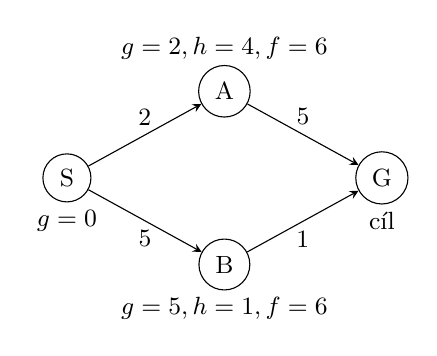
\begin{tikzpicture}[>=stealth, every node/.style={font=\small}]
        \node[draw,circle] (s) at (0,0) {S};
        \node[draw,circle] (a) at (2,1.1) {A};
        \node[draw,circle] (b) at (2,-1.1) {B};
        \node[draw,circle] (g) at (4,0) {G};
        \draw[->] (s)--node[above]{2}(a);
        \draw[->] (s)--node[below]{5}(b);
        \draw[->] (a)--node[above]{5}(g);
        \draw[->] (b)--node[below]{1}(g);
        \node at (0,-0.55) {\(g=0\)};
        \node at (2,1.65) {\(g=2,h=4,f=6\)};
        \node at (2,-1.65) {\(g=5,h=1,f=6\)};
        \node at (4,-0.55) {cíl};
    \end{tikzpicture}
    \caption{A* vybírá podle \(f=g+h\). Stejné \(f\) může vzniknout z levné cesty s horším odhadem i dražší cesty blíže k cíli.}
\end{figure}

\subsection*{Pokročilé varianty}
\begin{itemize}
    \item \textbf{Bidirectional A*} -- hledá současně od startu a od cíle. Výhoda je menší prohledaný prostor, omezení je nutnost znát reverzní operátory a správně řešit bod setkání.
    \item \textbf{Hierarchical A*} -- nejdříve plánuje v hrubém grafu a pak zpřesňuje cestu v detailech. Hodí se pro mapy, navigaci a robotiku.
\end{itemize}

\section{Biologicky inspirované výpočty: rozdělení a principy evolučních a rojových algoritmů (GA, DE, PSO, ACO, GP), lokální optimalizační metody (HC, HC-12, SA), reprezentace a kódování řešení, surrogate optimalizace, teorie no free lunch, prokletí dimenzionality, příklady problémů v AI.}

\subsection*{Co jsou bio-inspired algoritmy}
Bio-inspired algoritmy jsou optimalizační metody inspirované přírodními
procesy. Většinou jsou:
\begin{itemize}
    \item populační,
    \item stochastické,
    \item použitelné pro black-box funkce,
    \item bez potřeby derivací.
\end{itemize}

Důležitý pojem je \textbf{diverzita}. Znamená, jak moc se jedinci v populaci
liší. Malá diverzita vede k předčasné konvergenci, velká diverzita může
zpomalit nalezení přesného řešení.

\subsection*{Optimalizační úloha}
Optimalizační úloha je hledání nejlepšího řešení podle zadaného kritéria:
\begin{equation}
    x^* = \operatorname*{arg\,min}_{x \in \Omega} f(x)
\end{equation}
\begin{itemize}
    \item \(f(x)\) -- cílová funkce, kterou minimalizujeme nebo maximalizujeme.
    \item \(\Omega\) -- přípustná množina, tedy řešení splňující omezení.
    \item globální optimum -- nejlepší řešení v celé \(\Omega\).
    \item lokální optimum -- nejlepší řešení jen ve svém okolí.
\end{itemize}

\subsection*{Heuristika, metaheuristika, stochastičnost}
\textbf{Heuristika} je pravidlo pro konkrétní typ úloh. Využívá znalost struktury úlohy.

\textbf{Metaheuristika} je obecnější rámec použitelný na širokou třídu úloh. Typicky jen říká, jak generovat, měnit a vybírat kandidátní řešení.

\textbf{Stochastická metoda} používá náhodné veličiny. Výhoda je únik z lokálních minim, nevýhoda je pomalejší a neopakovatelný výsledek bez pevného seedu.

\textbf{Derivative-free metoda} nepotřebuje derivace ani analytický tvar funkce. Hodí se pro simulace, měření a black-box úlohy.

\subsection*{Explorace a exploatace}
\begin{itemize}
    \item \textbf{Explorace} -- globální průzkum prostoru, hledání nových oblastí.
    \item \textbf{Exploatace} -- lokální zlepšování v okolí dobrých řešení.
\end{itemize}

Příklady:
\begin{itemize}
    \item mutace v GA podporuje exploraci,
    \item křížení v GA podporuje exploataci dobrých částí řešení,
    \item vysoká teplota v SA podporuje exploraci,
    \item nízká teplota v SA podporuje exploataci,
    \item vyšší inerční váha v PSO podporuje průzkum.
\end{itemize}

\subsection*{Obecný rámec metaheuristiky}
\begin{figure}[H]
    \centering
    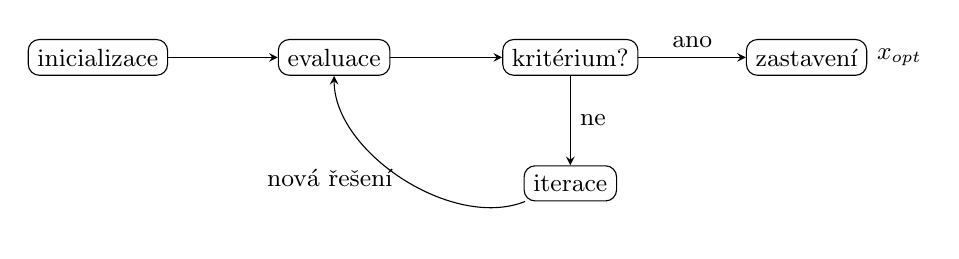
\begin{tikzpicture}[>=stealth, node distance=1.5cm, every node/.style={font=\small}]
        \node[draw,rounded corners] (init) at (0,0) {inicializace};
        \node[draw,rounded corners] (eval) at (3,0) {evaluace};
        \node[draw,rounded corners] (crit) at (6,0) {kritérium?};
        \node[draw,rounded corners] (stop) at (9,0) {zastavení};
        \node[draw,rounded corners] (iter) at (6,-1.6) {iterace};
        \draw[->] (init)--(eval);
        \draw[->] (eval)--(crit);
        \draw[->] (crit)--node[above]{ano}(stop);
        \draw[->] (crit)--node[right]{ne}(iter);
        \draw[->] (iter) .. controls (4.5,-2.2) and (3,-1.2) .. node[left]{nová řešení} (eval);
        \node[right] at (stop.east) {\(x_{opt}\)};
    \end{tikzpicture}
    \caption{Obecný tok metaheuristiky: generuj, ohodnoť, upravuj a zastav podle kritéria.}
\end{figure}

\subsection*{Reprezentace řešení}
\begin{itemize}
    \item \textbf{Binární} -- geny jsou 0/1, např. výběr prvků nebo klasický GA.
    \item \textbf{Reálná} -- geny jsou reálná čísla, např. spojitá optimalizace parametrů.
    \item \textbf{Permutační} -- řešení je pořadí prvků, např. TSP.
    \item \textbf{Stromová} -- řešení je strom programu/výrazu, např. genetické programování.
\end{itemize}

\textbf{Genotyp} je fyzické kódování proměnných, tedy to, s čím algoritmus pracuje. \textbf{Fenotyp} je výsledná interpretace řešení v reálné úloze.

Omezení lze řešit:
\begin{itemize}
    \item penalizací -- ke špatnému řešení přičtu trest,
    \item repair mechanismem -- po vygenerování řešení opravím do přípustné množiny,
    \item speciálním operátorem -- generuje jen platná řešení.
\end{itemize}

Zastavovací kritéria: počet iterací, počet evaluací fitness, dosažení
tolerance, stagnace nebo vyčerpání času. U black-box úloh je nejférovější
limitovat počet evaluací.

\subsection*{Premature convergence}
Premature convergence je předčasné uvíznutí v jedné oblasti prostoru. Pozná se
tak, že fitness se přestane zlepšovat a populace ztratí diverzitu.

Ochrana:
\begin{itemize}
    \item zvýšit mutaci,
    \item slabší selekční tlak,
    \item zachovat diverzitu populace,
    \item restart části populace,
    \item hybridizace s jinou metodou.
\end{itemize}

\subsection*{Genetický algoritmus (GA)}
GA pracuje s populací řešení. Lepší jedinci mají větší šanci předat vlastnosti
do další generace.

\begin{figure}[H]
    \centering
    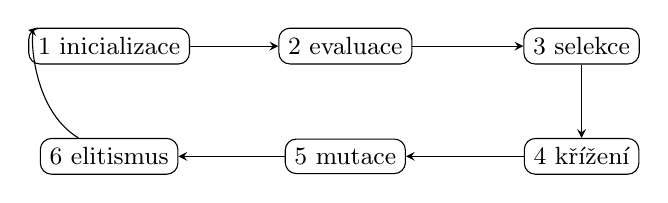
\begin{tikzpicture}[>=stealth, every node/.style={font=\small}]
        \node[draw,rounded corners] (i) at (0,0) {1 inicializace};
        \node[draw,rounded corners] (e) at (3,0) {2 evaluace};
        \node[draw,rounded corners] (s) at (6,0) {3 selekce};
        \node[draw,rounded corners] (c) at (6,-1.4) {4 křížení};
        \node[draw,rounded corners] (m) at (3,-1.4) {5 mutace};
        \node[draw,rounded corners] (el) at (0,-1.4) {6 elitismus};
        \draw[->] (i)--(e);
        \draw[->] (e)--(s);
        \draw[->] (s)--(c);
        \draw[->] (c)--(m);
        \draw[->] (m)--(el);
        \draw[->] (el) .. controls (-1,-0.8) and (-1,0.2) .. (i);
    \end{tikzpicture}
    \caption{Cyklus jedné generace genetického algoritmu.}
\end{figure}

Selekce:
\begin{itemize}
    \item \textbf{ruleta} -- pravděpodobnost výběru je úměrná fitness.
    \item \textbf{turnaj} -- vybere se několik jedinců a z nich nejlepší.
    \item \textbf{ranking} -- jedinci se řadí podle pořadí, ne podle absolutní fitness.
    \item \textbf{elitismus} -- nejlepší jedinci se přímo zachovají.
\end{itemize}

Selekční tlak říká, jak silně algoritmus zvýhodňuje nejlepší jedince. Silný
tlak rychle zlepšuje populaci, ale snižuje diverzitu.

\textbf{Křížení} kombinuje dva rodiče. Jednobodové křížení:
\begin{equation}
    111|00,\quad 000|11 \quad \Rightarrow \quad 11111,\quad 00000
\end{equation}
\textbf{Mutace} náhodně změní gen, např. bit-flip \(0 \leftrightarrow 1\), a udržuje diverzitu.

Pro permutační úlohy se používá OX/PMX křížení a mutace swap, insertion nebo
inversion, aby zůstala platná permutace.

Parametry:
\begin{itemize}
    \item \(N\) -- velikost populace; větší \(N\) zvyšuje diverzitu i výpočetní náročnost.
    \item \(P_c\) -- pravděpodobnost křížení; vyšší hodnota zvyšuje kombinování dobrých částí.
    \item \(P_m\) -- pravděpodobnost mutace; příliš malá vede ke stagnaci, příliš velká ničí dobrá řešení.
    \item elitismus -- počet zachovaných nejlepších jedinců.
\end{itemize}

\subsection*{Simulated Annealing (SA) a Hill Climbing}
Hill Climbing vždy vezme lepšího souseda. Je rychlý, ale snadno uvázne v
lokálním minimu, na plató nebo v hřebeni.

SA je jednoprvková stochastická metoda. Občas přijme i horší řešení, aby
přeskočila lokální minimum. Metropolisovo kritérium:
\begin{equation}
    P(\text{přijmout horší})=\exp\left(-\frac{\Delta f}{T}\right)
\end{equation}
Při vysoké teplotě \(T\) se horší řešení přijímají častěji, při nízké teplotě
se metoda chová podobně jako Hill Climbing.

\begin{figure}[H]
    \centering
    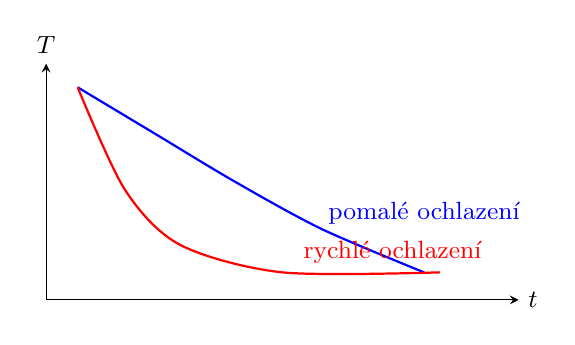
\begin{tikzpicture}[>=stealth, every node/.style={font=\small}]
        \draw[->] (0,0) -- (6,0) node[right]{\(t\)};
        \draw[->] (0,0) -- (0,3) node[above]{\(T\)};
        \draw[thick,blue] plot[smooth] coordinates {(0.4,2.7) (1.4,2.1) (2.4,1.5) (3.5,0.9) (4.8,0.35)};
        \draw[thick,red] plot[smooth] coordinates {(0.4,2.7) (1.0,1.4) (1.7,0.7) (3.0,0.35) (5.0,0.35)};
        \node[blue] at (4.8,1.1) {pomalé ochlazení};
        \node[red] at (4.4,0.6) {rychlé ochlazení};
    \end{tikzpicture}
    \caption{Pomalé ochlazování lépe prozkoumá prostor, rychlé ochlazování šetří čas, ale zvyšuje riziko lokálního minima.}
\end{figure}

SA se hodí pro TSP, scheduling, hledání minim v nespojitých prostorech a
embedded systémy s omezenou pamětí.

\subsection*{Differential Evolution (DE)}
DE je populační metoda pro reálné vektory. Je jednoduchá, má málo parametrů a
dobře funguje pro spojitou optimalizaci.

Mutace DE/rand/1:
\begin{equation}
    v_i = x_{r1} + F(x_{r2}-x_{r3})
\end{equation}
kde \(F\) škáluje rozdíl dvou vektorů. Potom se provede křížení s aktuálním
řešením podle \(CR\) a vybere se lepší kandidát.

\begin{figure}[H]
    \centering
    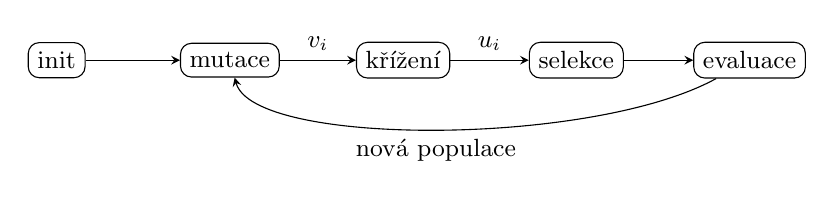
\begin{tikzpicture}[>=stealth, every node/.style={font=\small}]
        \node[draw,rounded corners] (init) at (0,0) {init};
        \node[draw,rounded corners] (mut) at (2.2,0) {mutace};
        \node[draw,rounded corners] (cross) at (4.4,0) {křížení};
        \node[draw,rounded corners] (sel) at (6.6,0) {selekce};
        \node[draw,rounded corners] (eval) at (8.8,0) {evaluace};
        \draw[->] (init)--(mut);
        \draw[->] (mut)--node[above]{\(v_i\)}(cross);
        \draw[->] (cross)--node[above]{\(u_i\)}(sel);
        \draw[->] (sel)--(eval);
        \draw[->] (eval) .. controls (6.8,-1.1) and (2.5,-1.1) .. node[below]{nová populace} (mut);
    \end{tikzpicture}
    \caption{Krok DE: diferenční mutace, křížení a výběr lepšího řešení.}
\end{figure}

Oproti GA pracuje DE přirozeně s reálnými vektory a mutace je založena na
rozdílu vektorů, ne jen na náhodné změně genu.

\subsection*{Particle Swarm Optimization (PSO)}
PSO je inspirováno hejnem. Každá částice má polohu \(x_i\), rychlost \(v_i\),
osobní nejlepší polohu \(p_i\) a globální nejlepší polohu \(g\).
\begin{equation}
    v_i(t+1)=\omega v_i(t)+c_1 r_1(p_i-x_i(t))+c_2 r_2(g-x_i(t))
\end{equation}
\begin{equation}
    x_i(t+1)=x_i(t)+v_i(t+1)
\end{equation}

\begin{figure}[H]
    \centering
    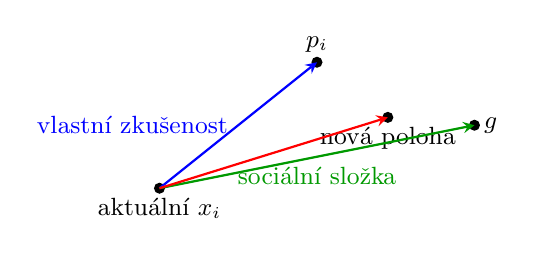
\begin{tikzpicture}[>=stealth, every node/.style={font=\small}]
        \coordinate (x) at (0,0);
        \coordinate (p) at (2,1.6);
        \coordinate (g) at (4,0.8);
        \coordinate (new) at (2.9,0.9);
        \fill (x) circle (2pt) node[below]{aktuální \(x_i\)};
        \fill (p) circle (2pt) node[above]{\(p_i\)};
        \fill (g) circle (2pt) node[right]{\(g\)};
        \fill (new) circle (2pt) node[below]{nová poloha};
        \draw[->,blue,thick] (x)--node[left]{vlastní zkušenost}(p);
        \draw[->,green!60!black,thick] (x)--node[below]{sociální složka}(g);
        \draw[->,red,thick] (x)--(new);
    \end{tikzpicture}
    \caption{PSO kombinuje setrvačnost, osobní nejlepší zkušenost a nejlepší zkušenost roje.}
\end{figure}

\subsection*{Ant Colony Optimization (ACO)}
ACO využívá stigmergii, tedy nepřímou komunikaci přes prostředí. Mravenci
konstruují řešení podle feromonové stopy a lokální heuristiky.
\begin{equation}
    p_{ij}=\frac{\tau_{ij}^{\alpha}\eta_{ij}^{\beta}}{\sum_{k \in N_i}\tau_{ik}^{\alpha}\eta_{ik}^{\beta}}
\end{equation}
\(\tau_{ij}\) je feromon -- zkušenost z minulých běhů. \(\eta_{ij}\) je heuristika -- lokální rada, např. převrácená vzdálenost. Čím lepší cesta, tím více feromonu se posílí. Část feromonu se zároveň odpařuje, aby algoritmus nezamrzl.

\subsection*{Další metody a srovnání}
\begin{itemize}
    \item \textbf{GP} -- genetické programování, jedinec je program nebo výraz ve stromu.
    \item \textbf{HC-12} -- kombinuje Hill Climbing s explorací, typicky pro binární prostor.
    \item \textbf{Populační metody} -- GA, DE, PSO, ACO; lépe paralelizovatelné, větší paměť.
    \item \textbf{Jednoprvkové metody} -- SA, HC; malá paměť, menší diverzita.
\end{itemize}

\subsection*{Vícekriteriální a surrogate optimalizace}
Vícekriteriální optimalizace má více cílů najednou. Řešení \(A\) dominuje
řešení \(B\), pokud není horší v žádném cíli a alespoň v jednom je lepší.
Pareto-fronta je množina nedominovaných kompromisů.

Surrogate optimalizace se používá, když je výpočet \(f(x)\) drahý. Místo něj se
učí levnější model:
\begin{equation}
    \hat f(x) \approx f(x)
\end{equation}
Ten navrhuje kandidáty a pravá funkce se volá jen pro vybrané body. Hodí se pro
simulace, FEM/CFD, experimenty nebo návrh parametrů.

\subsection*{Fair porovnání, konvergence, NFL}
Férové porovnání dvou metaheuristik:
\begin{itemize}
    \item stejný počet evaluací,
    \item více nezávislých běhů,
    \item stejný benchmark a omezení,
    \item reportovat průměr, rozptyl a nejlepší výsledek.
\end{itemize}

Konvergence se v praxi chápe jako stabilizace fitness nebo vyčerpání rozpočtu.
Globální optimum většinou garantované není.

\textbf{No Free Lunch theorem}: žádný algoritmus není nejlepší pro všechny možné úlohy. Metodu je nutné vybírat podle typu problému.

\textbf{Prokletí dimenzionality}: s růstem počtu proměnných roste prostor řešení extrémně rychle. Stejná hustota vzorkování vyžaduje mnohem více evaluací.

\textbf{Hollandův schema theorem}: krátká, málo narušená a nadprůměrně kvalitní schémata mají tendenci se v populaci šířit.

\begin{equation}
    H = 1 * 0 * * 1
\end{equation}
je schéma, kde hvězdička znamená libovolný gen.

\section{Neuronové sítě – vybraná základní paradigmata: formální neuron, aktivační funkce, architektury (perceptron, ADALINE, MLP, RBF, SOM), učení (včetně zpětného šíření chyby), klasifikace a regrese, problémy učení (overfitting, kapacita), příklady problémů v AI.}

\subsection*{Paradigmata učení}
Paradigma učení říká, jak model chápe proces učení.

\begin{center}
    \begin{tabularx}{\textwidth}{|l|X|}
        \hline
        \textbf{Učení s učitelem}  & data jsou označená, model se učí mapovat vstup na správný výstup; typicky klasifikace a regrese  \\
        \hline
        \textbf{Učení bez učitele} & data nejsou označená, model hledá strukturu; typicky shlukování a redukce dimenze                \\
        \hline
        \textbf{Posilované učení}  & agent zkouší akce v prostředí a dostává odměny/tresty; cílem je maximalizovat dlouhodobou odměnu \\
        \hline
    \end{tabularx}
\end{center}

\textbf{Architektura} je struktura sítě: počet vrstev, počet neuronů, propojení a aktivační funkce. \textbf{Učení vah} je hledání hodnot vah a biasů tak, aby síť dávala správné výstupy.

\begin{itemize}
    \item \textbf{Parametry} -- váhy a biasy, model se je učí sám.
    \item \textbf{Hyperparametry} -- nastavení zvenku: počet vrstev, learning rate, batch size, optimalizátor.
\end{itemize}

\subsection*{Biologická inspirace a formální neuron}
Biologický neuron má dendrity, somu a axon. Dendrity přijímají signály, soma je
integruje a axon posílá výstup dál. Synapse je spoj mezi neurony, může být
excitační nebo inhibiční.

Umělý neuron je zjednodušenina: vstupy se vynásobí vahami, sečtou, přičte se
bias a výsledek jde přes aktivační funkci.

\begin{figure}[H]
    \centering
    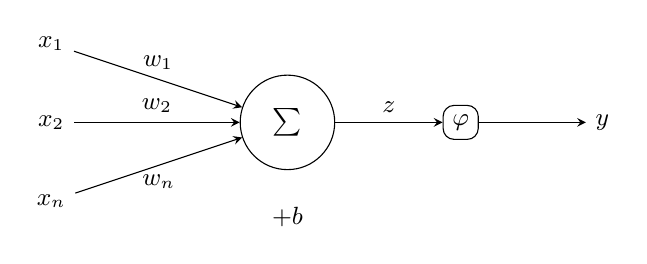
\begin{tikzpicture}[>=stealth, every node/.style={font=\small}]
        \node (x1) at (0,1) {\(x_1\)};
        \node (x2) at (0,0) {\(x_2\)};
        \node (xn) at (0,-1) {\(x_n\)};
        \node[draw,circle,minimum size=1.2cm] (sum) at (3,0) {\(\sum\)};
        \node[draw,rounded corners] (act) at (5.2,0) {\(\varphi\)};
        \node (y) at (7,0) {\(y\)};
        \draw[->] (x1)--node[above]{\(w_1\)}(sum);
        \draw[->] (x2)--node[above]{\(w_2\)}(sum);
        \draw[->] (xn)--node[below]{\(w_n\)}(sum);
        \node at (3,-1.2) {\(+b\)};
        \draw[->] (sum)--node[above]{\(z\)}(act);
        \draw[->] (act)--(y);
    \end{tikzpicture}
    \caption{Formální neuron: vážený součet, bias a aktivační funkce.}
\end{figure}

\begin{equation}
    z=b+\sum_{i=1}^{n}w_i x_i,\qquad y=\varphi(z)
\end{equation}

Akční potenciál u biologického neuronu je impuls 0/1 a intenzita se kóduje
frekvencí impulsů. Výstup umělého neuronu je číslo, jehož velikost přímo nese
informaci.

\subsection*{Aktivační funkce}
\begin{itemize}
    \item \textbf{step} -- tvrdé rozhodnutí 0/1 nebo -1/1.
    \item \textbf{sigmoid} -- výstup \(0\) až \(1\), vhodný pro pravděpodobnost binární třídy.
    \item \textbf{tanh} -- výstup \(-1\) až \(1\).
    \item \textbf{ReLU} -- \(\max(0,x)\), jednoduchá a vhodná pro hluboké sítě.
    \item \textbf{softmax} -- převede výstupní vektor na pravděpodobnosti tříd.
\end{itemize}

\subsection*{Perceptron}
Perceptron je nejjednodušší neuronová síť pro lineární klasifikaci. Rozhoduje
pomocí nadroviny:
\begin{equation}
    w^T x + b = 0
\end{equation}
Učící pravidlo:
\begin{equation}
    w_i(t+1)=w_i(t)+\alpha(d-y)x_i
\end{equation}

Umí řešit lineárně separabilní úlohy. Neumí XOR, protože XOR nelze rozdělit
jednou přímkou nebo jednou nadrovinou.

\begin{figure}[H]
    \centering
    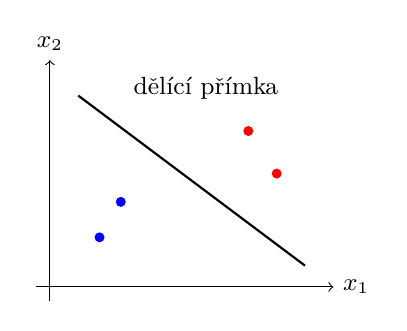
\begin{tikzpicture}[scale=0.9, every node/.style={font=\small}]
        \draw[->] (-0.2,0)--(4,0) node[right]{\(x_1\)};
        \draw[->] (0,-0.2)--(0,3.2) node[above]{\(x_2\)};
        \fill[blue] (0.7,0.7) circle (2pt);
        \fill[blue] (1.0,1.2) circle (2pt);
        \fill[red] (2.8,2.2) circle (2pt);
        \fill[red] (3.2,1.6) circle (2pt);
        \draw[thick] (0.4,2.7)--(3.6,0.3);
        \node at (2.2,2.8) {dělící přímka};
    \end{tikzpicture}
    \caption{Lineárně separabilní data lze oddělit jednou přímkou.}
\end{figure}

\subsection*{ADALINE}
ADALINE je Adaptive Linear Neuron. Oproti perceptronu se učí podle lineární
odezvy před prahováním a minimalizuje kvadratickou chybu.
\begin{equation}
    w_i(t+1)=w_i(t)+\alpha(d-z)x_i
\end{equation}
Výhoda je hladký chybový povrch pro lineární model. Učení lze chápat jako
gradientní sestup nad MSE.

\subsection*{MLP a backpropagation}
MLP je vícevrstvá dopředná síť. Má vstupní vrstvu, jednu nebo více skrytých
vrstev a výstupní vrstvu. Nelineární aktivační funkce umožní řešit i nelineárně
separabilní úlohy.

\begin{figure}[H]
    \centering
    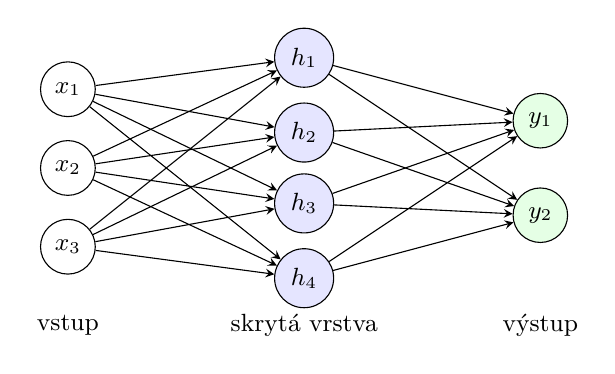
\begin{tikzpicture}[>=stealth, every node/.style={font=\small}]
        \node[draw,circle] (i1) at (0,1) {\(x_1\)};
        \node[draw,circle] (i2) at (0,0) {\(x_2\)};
        \node[draw,circle] (i3) at (0,-1) {\(x_3\)};

        \node[draw,circle,fill=blue!10] (h1) at (3,1.4) {\(h_1\)};
        \node[draw,circle,fill=blue!10] (h2) at (3,0.45) {\(h_2\)};
        \node[draw,circle,fill=blue!10] (h3) at (3,-0.45) {\(h_3\)};
        \node[draw,circle,fill=blue!10] (h4) at (3,-1.4) {\(h_4\)};

        \node[draw,circle,fill=green!10] (o1) at (6,0.6) {\(y_1\)};
        \node[draw,circle,fill=green!10] (o2) at (6,-0.6) {\(y_2\)};

        \foreach \a in {i1,i2,i3} {
                \foreach \b in {h1,h2,h3,h4} {
                        \draw[->] (\a)--(\b);
                    }
            }
        \foreach \a in {h1,h2,h3,h4} {
                \foreach \b in {o1,o2} {
                        \draw[->] (\a)--(\b);
                    }
            }
        \node at (0,-2) {vstup};
        \node at (3,-2) {skrytá vrstva};
        \node at (6,-2) {výstup};
    \end{tikzpicture}
    \caption{MLP: více vrstev a úplné propojení mezi sousedními vrstvami.}
\end{figure}

Backpropagation:
\begin{enumerate}
    \item dopředně spočítá výstup,
    \item spočítá chybu,
    \item chybu šíří zpět přes vrstvy,
    \item upraví váhy podle gradientu.
\end{enumerate}
\begin{equation}
    w(t+1)=w(t)-\alpha\frac{\partial E}{\partial w}
\end{equation}

Learning rate \(\alpha\) určuje velikost kroku. Příliš velká hodnota rozkmitá
učení, příliš malá učení zpomalí.

\subsection*{Loss funkce a režimy učení}
\begin{itemize}
    \item regrese -- často MSE,
          \begin{equation}
              E=\frac{1}{m}\sum_{i=1}^{m}(y_i-d_i)^2
          \end{equation}
    \item klasifikace -- často cross-entropy.
\end{itemize}

\begin{itemize}
    \item \textbf{batch} -- aktualizace po celé trénovací množině.
    \item \textbf{mini-batch} -- aktualizace po menší dávce, nejběžnější.
    \item \textbf{online / stochastic} -- aktualizace po jednom vzoru.
\end{itemize}

\subsection*{RBF sítě}
RBF síť používá radiální aktivační funkce. Skrytý neuron reaguje hlavně na
vzory blízko svého centra:
\begin{equation}
    \phi_j(x)=\exp\left(-\frac{\|x-c_j\|^2}{2\sigma_j^2}\right)
\end{equation}

Učení bývá dvoufázové:
\begin{itemize}
    \item neřízeně se najdou centra a šířky, např. k-means,
    \item řízeně se naučí výstupní lineární váhy.
\end{itemize}

K-means:
\begin{enumerate}
    \item náhodně zvol centra shluků,
    \item přiřaď body k nejbližšímu centru,
    \item přepočítej centra jako průměr bodů,
    \item opakuj do ustálení.
\end{enumerate}

MLP se učí globální nelineární transformaci, RBF je lokálnější a hodně závisí
na rozmístění center.

\subsection*{Samoorganizační mapy (SOM)}
SOM je učení bez učitele. Neurony ve výstupní mapě soutěží o vstupní vzor.
Vítězný neuron je BMU:
\begin{equation}
    BMU=\operatorname*{arg\,min}_{j}\|x-w_j\|
\end{equation}
Strategie Winner-Takes-All znamená, že aktivní je hlavně vítěz. Laterální
inhibice znamená potlačení vzdálenějších neuronů.

Váhy vítěze a jeho okolí se posunou ke vstupu:
\begin{equation}
    w_j(t+1)=w_j(t)+\alpha(t)h_{bj}(t)(x-w_j(t))
\end{equation}

Funkce sousedství určuje, jak moc se učí okolní neurony. Na začátku je okolí
velké, později se zmenšuje. Topologické zachování znamená, že podobné vstupy
leží v mapě blízko sebe.

\begin{figure}[H]
    \centering
    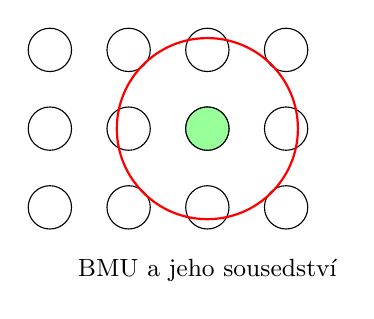
\begin{tikzpicture}[every node/.style={font=\small}]
        \foreach \x in {0,1,2,3} {
                \foreach \y in {0,1,2} {
                        \node[draw,circle,minimum size=0.55cm] (n\x\y) at (\x,\y) {};
                    }
            }
        \node[draw,circle,fill=green!40,minimum size=0.55cm] at (2,1) {};
        \draw[red,thick] (2,1) circle (1.15cm);
        \node at (2,-0.8) {BMU a jeho sousedství};
    \end{tikzpicture}
    \caption{SOM: vítězný neuron a jeho okolí se posouvají ke vstupnímu vzoru.}
\end{figure}

\subsection*{Klasifikace, regrese a problémy učení}
Klasifikace zařazuje vstup do tříd. Regrese odhaduje spojitou hodnotu.

\begin{itemize}
    \item \textbf{Overfitting} -- síť se naučí trénovací data moc přesně a neumí generalizovat.
    \item \textbf{Underfitting} -- síť je moc jednoduchá nebo špatně naučená.
    \item \textbf{Kapacita} -- schopnost sítě reprezentovat složitou funkci. Roste s počtem vrstev, neuronů a parametrů.
\end{itemize}

Proti overfittingu: regularizace, dropout, early stopping, více dat,
augmentace, menší model.

\section{Neuronové sítě – vybraná DNN paradigmata: architektury (CNN - podrobně; RNN, Encoder-Decoder, Transformer - přehledově), aktivační funkce, princip učení, implementace (Keras) a trénink DNN, příklady problémů v AI.}

\subsection*{Hluboká neuronová síť}
DNN má více skrytých vrstev. Nižší vrstvy zachycují jednoduché rysy, vyšší
vrstvy skládají složitější reprezentace.

Problémy hloubky:
\begin{itemize}
    \item \textbf{vanishing gradient} -- gradient se zmenšuje a nižší vrstvy se skoro neučí.
    \item \textbf{exploding gradient} -- gradient roste a učení je nestabilní.
    \item \textbf{overfitting} -- mnoho parametrů vůči malému datasetu.
\end{itemize}

Řešení: ReLU/GeLU, vhodná inicializace, normalizace, reziduální spojení, regularizace.

\subsection*{Softmax a cross-entropy}
Softmax převádí skóre tříd na pravděpodobnosti:
\begin{equation}
    softmax(z)_i=\frac{e^{z_i}}{\sum_j e^{z_j}}
\end{equation}
Cross-entropy trestá nízkou pravděpodobnost správné třídy:
\begin{equation}
    L=-\sum_i y_i\log(\hat y_i)
\end{equation}
V klasifikaci se softmax a cross-entropy používají společně, protože výstup lze
chápat pravděpodobnostně.

\subsection*{CNN}
CNN je síť pro data s lokální strukturou, hlavně obraz. Oproti plně propojené
síti má:
\begin{itemize}
    \item lokální receptivní pole,
    \item sdílení vah,
    \item výrazně méně parametrů,
    \item lepší práci s posunem objektu v obraze.
\end{itemize}

Konvoluční filtr prochází obraz a vytváří mapu příznaků:
\begin{equation}
    y(i,j)=\sum_u\sum_v k(u,v)x(i+u,j+v)+b
\end{equation}

\begin{figure}[H]
    \centering
    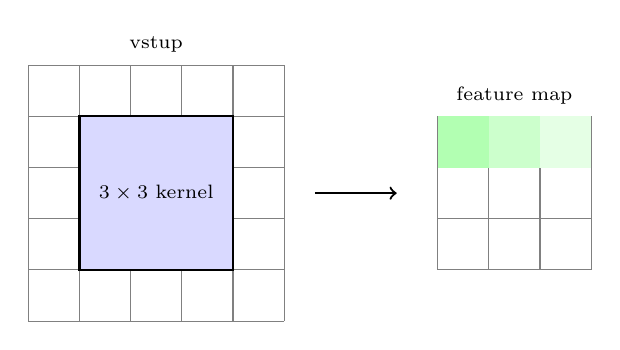
\begin{tikzpicture}[scale=0.65, every node/.style={font=\scriptsize}]
        \draw[step=1cm,gray] (0,0) grid (5,5);
        \draw[fill=blue!15,thick] (1,1) rectangle (4,4);
        \node at (2.5,5.4) {vstup};
        \node at (2.5,2.5) {\(3\times3\) kernel};
        \draw[->,thick] (5.6,2.5)--(7.2,2.5);
        \draw[step=1cm,gray] (8,1) grid (11,4);
        \node at (9.5,4.4) {feature map};
        \fill[green!30] (8,3) rectangle (9,4);
        \fill[green!20] (9,3) rectangle (10,4);
        \fill[green!10] (10,3) rectangle (11,4);
    \end{tikzpicture}
    \caption{Konvoluce: jeden filtr se posouvá po vstupu a tvoří mapu příznaků.}
\end{figure}

Rozměr výstupu:
\begin{equation}
    N_{out}=\left\lfloor\frac{N+2P-F}{S}\right\rfloor+1
\end{equation}
kde \(P\) je padding, \(F\) velikost filtru a \(S\) stride.

Pooling zmenšuje rozměr a zvyšuje robustnost:
\begin{itemize}
    \item max pooling -- bere maximum.
    \item average pooling -- bere průměr.
\end{itemize}

Typická CNN:
\begin{equation}
    \text{konvoluce} \rightarrow \text{aktivace} \rightarrow \text{pooling} \rightarrow \text{fully-connected}
\end{equation}

Známé architektury: LeNet, AlexNet, VGG, ResNet. Použití: klasifikace obrazu,
detekce objektů, segmentace, kontrola kvality, medicínské snímky.

\subsection*{RNN, LSTM, GRU}
RNN zpracovává sekvenci postupně a drží skrytý stav:
\begin{equation}
    h_t=\varphi(W_xx_t+W_hh_{t-1}+b)
\end{equation}

\begin{figure}[H]
    \centering
    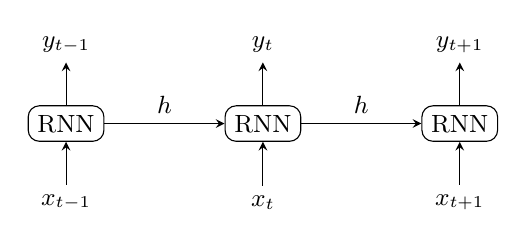
\begin{tikzpicture}[>=stealth, every node/.style={font=\small}]
        \node[draw,rounded corners] (r1) at (0,0) {RNN};
        \node[draw,rounded corners] (r2) at (2.5,0) {RNN};
        \node[draw,rounded corners] (r3) at (5,0) {RNN};
        \node (x1) at (0,-1) {\(x_{t-1}\)};
        \node (x2) at (2.5,-1) {\(x_t\)};
        \node (x3) at (5,-1) {\(x_{t+1}\)};
        \node (y1) at (0,1) {\(y_{t-1}\)};
        \node (y2) at (2.5,1) {\(y_t\)};
        \node (y3) at (5,1) {\(y_{t+1}\)};
        \draw[->] (x1)--(r1); \draw[->] (x2)--(r2); \draw[->] (x3)--(r3);
        \draw[->] (r1)--(y1); \draw[->] (r2)--(y2); \draw[->] (r3)--(y3);
        \draw[->] (r1)--node[above]{\(h\)}(r2);
        \draw[->] (r2)--node[above]{\(h\)}(r3);
    \end{tikzpicture}
    \caption{RNN předává skrytý stav mezi časovými kroky.}
\end{figure}

Omezení RNN: špatně se učí dlouhé závislosti a trpí mizejícím/explodujícím
gradientem.

LSTM používá cell state a brány forget, input, output. GRU je jednodušší
varianta s update/reset branami. Obě architektury zlepšují práci s delší
pamětí.

\subsection*{Encoder--Decoder}
Encoder přečte vstupní sekvenci a vytvoří reprezentaci. Decoder z ní generuje
výstupní sekvenci. Používá se pro překlad, sumarizaci nebo speech-to-text.

Bez attention se dlouhá věta mačká do jednoho vektoru. Attention umožní
decoderu dívat se na různé části vstupu.

\subsection*{Transformer}
Transformer je architektura bez rekurence založená na self-attention.
\begin{equation}
    Attention(Q,K,V)=softmax\left(\frac{QK^T}{\sqrt{d_k}}\right)V
\end{equation}

\begin{itemize}
    \item \(Q\) -- queries, čím se token ptá.
    \item \(K\) -- keys, podle čeho se hledá shoda.
    \item \(V\) -- values, informace, která se přenáší.
\end{itemize}

\begin{figure}[H]
    \centering
    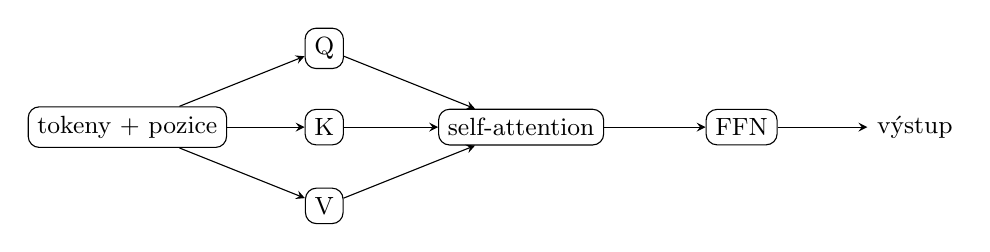
\begin{tikzpicture}[>=stealth, every node/.style={font=\small}]
        \node[draw,rounded corners] (x) at (0,0) {tokeny + pozice};
        \node[draw,rounded corners] (q) at (2.5,1) {Q};
        \node[draw,rounded corners] (k) at (2.5,0) {K};
        \node[draw,rounded corners] (v) at (2.5,-1) {V};
        \node[draw,rounded corners] (att) at (5,0) {self-attention};
        \node[draw,rounded corners] (ffn) at (7.8,0) {FFN};
        \node (out) at (10,0) {výstup};
        \draw[->] (x)--(q);
        \draw[->] (x)--(k);
        \draw[->] (x)--(v);
        \draw[->] (q)--(att);
        \draw[->] (k)--(att);
        \draw[->] (v)--(att);
        \draw[->] (att)--(ffn);
        \draw[->] (ffn)--(out);
    \end{tikzpicture}
    \caption{Základní tok v transformer bloku. Multi-head attention používá více takových pohledů paralelně.}
\end{figure}

Self-attention nezná pořadí, proto se přidává pozicové kódování.

\begin{itemize}
    \item \textbf{Encoder-only} -- BERT, vhodný pro klasifikaci a porozumění textu.
    \item \textbf{Decoder-only} -- GPT, autoregresivně generuje další token.
    \item \textbf{Encoder--Decoder} -- překlad, sumarizace, Seq2Seq.
\end{itemize}

Transformer proti RNN:
\begin{itemize}
    \item lépe paralelizovatelný,
    \item lépe pracuje s dlouhými závislostmi,
    \item self-attention má náročnost přibližně \(O(n^2)\) podle délky sekvence.
\end{itemize}

\subsection*{Trénink DNN a Keras}
Základní postup:
\begin{enumerate}
    \item definice architektury,
    \item volba loss funkce,
    \item volba optimalizátoru,
    \item trénování na trénovacích datech,
    \item kontrola validační chyby,
    \item test na testovacích datech.
\end{enumerate}

\begin{itemize}
    \item \textbf{epoch} -- jeden průchod trénovací množinou.
    \item \textbf{batch size} -- počet vzorů pro jeden krok učení.
    \item \textbf{learning rate} -- velikost kroku optimalizace.
\end{itemize}

\textbf{Sequential API} v Keras je pro jednoduchou lineární posloupnost vrstev. \textbf{Functional API} je pro více vstupů/výstupů, větvení a sdílení vrstev.

\begin{lstlisting}[language=Python]
model.compile(optimizer="adam",
              loss="sparse_categorical_crossentropy",
              metrics=["accuracy"])

model.fit(x_train, y_train,
          epochs=20,
          batch_size=64,
          validation_split=0.2)

model.evaluate(x_test, y_test)
\end{lstlisting}

\texttt{compile()} nastaví loss a optimalizátor. \texttt{fit()} trénuje. \texttt{evaluate()} vyhodnotí model.

Optimalizátory:
\begin{itemize}
    \item \textbf{SGD} -- jednoduchý gradientní sestup.
    \item \textbf{RMSprop} -- adaptuje krok podle velikosti gradientů.
    \item \textbf{Adam} -- kombinuje moment a adaptivní krok, v praxi velmi častý.
\end{itemize}

\subsection*{Příklady použití DNN}
Klasifikace obrazu, detekce objektů, segmentace, rozpoznávání řeči, strojový
překlad, sumarizace, generování textu, predikce časových řad, anomálie,
robotika a zpracování signálů.
